\section{PHƯƠNG PHÁP ĐỀ XUẤT}

\subsection{Tổng quan kiến trúc}

TrafficVision-Transformer được thiết kế như một biến thể nhẹ của hướng Spatio-Temporal Transformer đã được sử dụng trong phát hiện bất thường giao thông từ video trên không \cite{c1}. Đầu vào của mô hình là bốn khung hình liên tiếp $\{X_{t-4},X_{t-3},X_{t-2},X_{t-1}\}$ và đầu ra là khung hình dự đoán $\hat{X}_t$. Sau đó, sai số giữa $\hat{X}_t$ và khung hình thật $X_t$ được dùng làm điểm bất thường.

Pipeline gồm bốn khối chính:
\begin{itemize}
    \item \textbf{Data Loader}: tạo mẫu gồm năm frame liên tiếp, chuẩn hóa ảnh về miền $[-1,1]$ và sinh hai nhánh độ phân giải.
    \item \textbf{Spatial Transformer Encoder}: trích xuất token không gian đại diện cho từng frame.
    \item \textbf{Temporal Transformer Encoder}: học quan hệ chuyển động giữa các token frame.
    \item \textbf{Decoder}: tái tạo khung hình tương lai ở độ phân giải $256 \times 256$.
\end{itemize}

\begin{figure*}[t]
\centering
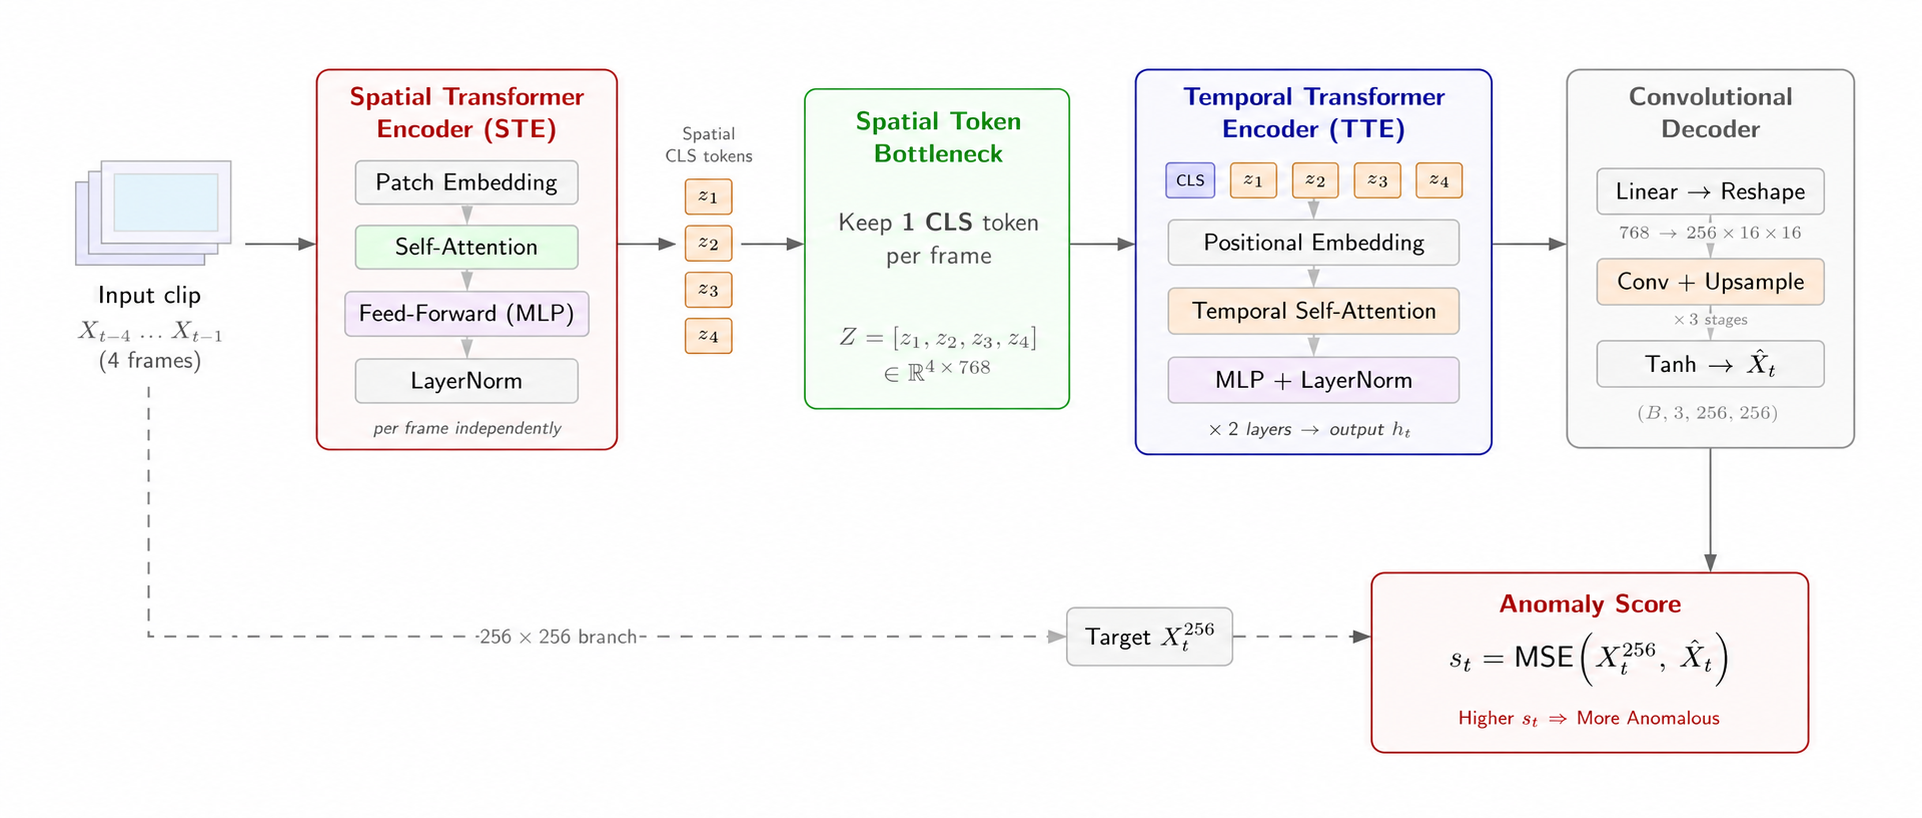
\includegraphics[width=\textwidth]{figures/pipeline.png}
\caption{Pipeline tổng quát của TrafficVision-Transformer. Sơ đồ nhấn mạnh điểm điều chỉnh chính của nhóm: Spatial Token Bottleneck giữ một token đại diện cho mỗi frame trước khi đưa vào Temporal Transformer Encoder, giúp giảm chi phí attention trong khi vẫn giữ thông tin chuyển động theo thời gian.}
\label{fig:pipeline}
\end{figure*}

Hình \ref{fig:pipeline} minh họa luồng xử lý tổng quát của mô hình. Điểm quan trọng là Temporal Transformer Encoder không nhận toàn bộ patch token của video, mà chỉ nhận một token đại diện cho mỗi frame. Nhờ đó, mô hình vẫn học được quan hệ thời gian nhưng giảm đáng kể chi phí attention.

\subsection{Tiền xử lý chuỗi frame}

Với mỗi video, các frame được sắp xếp theo thứ tự thời gian. Một mẫu huấn luyện gồm $T+1$ frame, trong đó $T=4$ frame đầu dùng làm đầu vào và frame cuối làm mục tiêu dự đoán. Trong project, mỗi frame được tạo ở hai kích thước:
\begin{itemize}
    \item Nhánh \texttt{standard}: dùng cho encoder, có kích thước cấu hình như $224$, $256$ hoặc $384$.
    \item Nhánh \texttt{256}: dùng làm mục tiêu tái tạo cho hàm mất mát MSE.
\end{itemize}

Thiết kế hai nhánh này giúp encoder vẫn có thể khai thác ảnh đầu vào độ phân giải cao hơn, trong khi decoder chỉ cần tái tạo ảnh $256 \times 256$ để giảm bộ nhớ và thời gian huấn luyện.

\subsection{Spatial Token Bottleneck: điểm điều chỉnh chính}

Nếu đưa toàn bộ patch token của mỗi frame vào Transformer thời gian, số token sẽ tăng nhanh theo độ phân giải ảnh. Ví dụ với ảnh $384 \times 384$ và patch size $32$, mỗi frame có $144$ patch token. Với bốn frame, attention thời gian trên toàn bộ patch token sẽ rất tốn tài nguyên.

Để giảm chi phí, nhóm sử dụng Spatial Token Bottleneck. Đây là điểm điều chỉnh chính so với cách xử lý video Transformer nặng hơn: thay vì để Temporal Encoder nhìn thấy toàn bộ patch token, mỗi frame $X_i$ đi qua Spatial Transformer Encoder và chỉ giữ một token đại diện:
\begin{equation}
z_i = STE(X_i), \quad z_i \in \mathbb{R}^{d}.
\end{equation}
Chuỗi bốn frame được biểu diễn thành ma trận:
\begin{equation}
Z = [z_{t-4}, z_{t-3}, z_{t-2}, z_{t-1}] \in \mathbb{R}^{T \times d}.
\end{equation}
Nhờ đó, Temporal Encoder chỉ xử lý số token tỉ lệ với số frame, không còn tỉ lệ với số patch trong ảnh. Với phạm vi seminar, lựa chọn này là thỏa hiệp hợp lý: mô hình có thể mất một phần chi tiết không gian nhỏ, nhưng đổi lại pipeline có thể chạy, debug và phân tích trên tài nguyên phổ thông.

\subsection{Temporal Transformer Encoder}

Để học quan hệ thời gian, một token \texttt{[CLS]} học được được thêm vào đầu chuỗi:
\begin{equation}
E = [z_{cls}, z_{t-4}, z_{t-3}, z_{t-2}, z_{t-1}].
\end{equation}
Sau đó, chuỗi này được đưa qua Temporal Transformer Encoder:
\begin{equation}
H = TTE(E).
\end{equation}
Vector tại vị trí \texttt{[CLS]} sau khi mã hóa, ký hiệu $h_t = H_0$, được dùng như biểu diễn tổng hợp của toàn bộ đoạn video ngắn. TTE trong mô hình được giữ nông để phù hợp tài nguyên tính toán và giảm nguy cơ huấn luyện quá lâu.

\subsection{Decoder và hàm mất mát}

Decoder nhận vector $h_t$ và tái tạo khung hình tương lai $\hat{X}_t$. Đầu tiên, $h_t$ được ánh xạ tuyến tính thành tensor đặc trưng, sau đó đi qua các lớp convolution và transposed convolution để sinh ảnh RGB $256 \times 256$.

Hàm mất mát huấn luyện là MSE reconstruction:
\begin{equation}
\mathcal{L}_{rec} = \frac{1}{N}\sum_{t=1}^{N}\left\|X_t^{256} - \hat{X}_t\right\|_2^2.
\end{equation}
Trong đó $X_t^{256}$ là khung hình thật đã resize về $256 \times 256$. Mô hình chỉ cần tối ưu khả năng tái tạo dữ liệu bình thường.

\subsection{Điểm bất thường và quyết định}

Ở giai đoạn suy luận, với mỗi thời điểm $t$, điểm bất thường được tính như sau:
\begin{equation}
s_t = MSE(X_t^{256}, \hat{X}_t).
\end{equation}
Điểm số càng cao thì khả năng bất thường càng lớn. Để so sánh giữa các video, có thể chuẩn hóa điểm số về $[0,1]$:
\begin{equation}
\tilde{s}_t = \frac{s_t-\min(s)}{\max(s)-\min(s)+\epsilon}.
\end{equation}
Trong cấu hình đơn giản, ngưỡng phát hiện được xác định theo trung bình và độ lệch chuẩn:
\begin{equation}
\tau = \mu_s + \sigma_s.
\end{equation}
Khung hình được dự đoán là bất thường nếu $s_t > \tau$.

\subsection{Thuật toán}

\subsection{Thuật toán huấn luyện}

Quy trình huấn luyện có thể tóm tắt như sau:
\begin{enumerate}
    \item Khởi tạo Spatial Transformer Encoder, Temporal Transformer Encoder và Decoder.
    \item Với mỗi batch, lấy chuỗi $X_{t-4:t}$ gồm năm frame liên tiếp.
    \item Đưa bốn frame đầu qua STE để thu được chuỗi token $Z$.
    \item Đưa $Z$ qua TTE để thu được biểu diễn tổng hợp $h_t$.
    \item Decoder sinh khung hình dự đoán $\hat{X}_t$.
    \item Tính $\mathcal{L}_{rec}=MSE(X_t^{256},\hat{X}_t)$ và cập nhật tham số bằng lan truyền ngược.
\end{enumerate}
